\section{Everything is Going Swimmingly!}

\instructornote{%
By Matt Trawick, 2019.  Time: 20 minutes

This lab assumes that students have already seen the Galilean transformations, for instance as developed at the end of the lab ``Galilean Relativity.''

This lab istwo quick problems involving swimming across a river.  In Activity 1, the first two parts are cribbed directly from Knight, 3rd edition, problem 4.17.  Activity 2, which involves swimming parallel vs. perpendicular to the current, is explicitly designed to prepare students for some future discussion of the Michelson-Morley experiment.  There's no particular reason to do this lab if you don't plan to mention the Michelson-Morley experiment.
}
\makelabheader %(Space for student name, etc., defined in master.tex or labmanual_formatting_commands.tex)

\textbf{Objective:}
\begin{itemize}
\item This lab steps through a couple of problems involving swimming in a river, either across the current of the water or parallel to it.  In fact, the race between Bob and Anna in Activity 2 is analagous to the famous ``Michaelson and Morley'' experiment, which involved sending light beams through the supposed ``lumeniferous ether,'' either across the current of the ether or parallel to it.
\end{itemize}

\textbf{Activity 1: Crossing a River} 

Problem 1: Anna can swim 2~m/s in still water.  She wants to swim across a river that flows east with a speed of 1~m/s.

\begin{enumerate}[labparts]
\item Suppose the river is 100~m wide.  If she aims directly north, how far downstream from her intended landing point will she end up?
\answerspace{0.6in}

\item What is her speed relative to the shore if she aims due north across the river, as in part (a)?
\answerspace{0.6in}

\hspace{\fill}\textit{Answer: 2.24~m/s}

\item What is her speed relative to the shore if she swims at an angle so that she ends up on the shore directly across from where she started?  Drawing a picture below will help.
\answerspace{0.6in}

\hspace{\fill}\textit{Answer: 1.73~m/s}

\end{enumerate}

\textbf{Activity 2: A swimming race} 

Anna and Bob can both swim at speed $v_s$ in still water.  They decide to have a race in a river of width $L$ that flows east at speed $v_r$.

\begin{minipage}{0.50 \textwidth}
\smallskip
\begin{itemize}
\item Anna swims across the river and back.  She swims at an angle to the current so she returns   exactly to her starting point.  (Anna swims north, then south.)
\item Bob swims downstream in the river with the current for a distance $L$ (relative to the shore), then swims back upstream against the current, also returning exactly to his starting point. (Bob swims east, then west).
\end{itemize}
\smallskip
\end{minipage}
\begin{minipage}{0.49 \textwidth}

\hspace{\fill}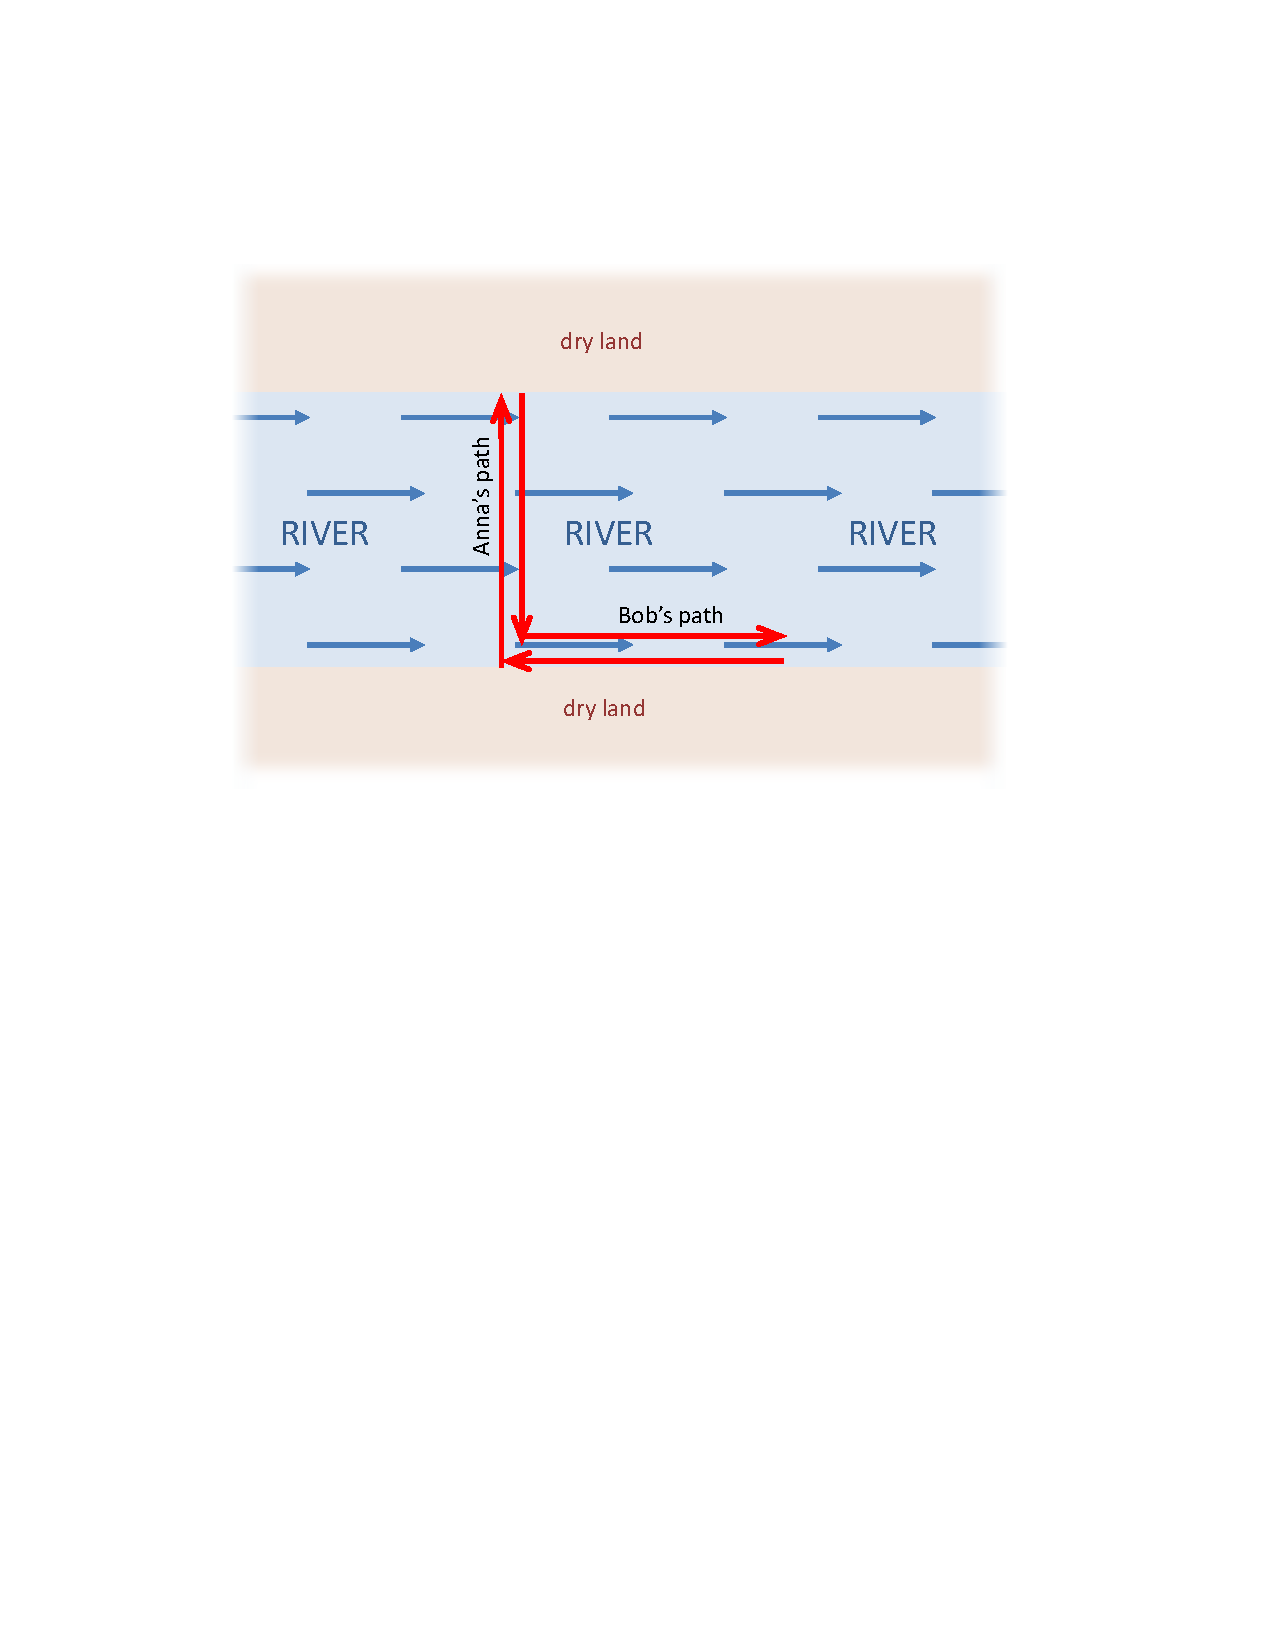
\includegraphics[scale=0.55]{swimming_race/river_diagram.pdf}
\index{color page}
\end{minipage}

\begin{enumerate}[labparts]

\item What is Anna's speed relative to the shore?
\answerspace{0.6in}

\hspace{\fill}\textit{Answer: $\sqrt{v_s^2-v_r^2}$}


\item What is Bob's speed relative to the shore when he swims downstream?  What is his speed relative to the shore when he swims upstream?
\answerspace{0.6in}

%\hspace{\fill}\textit{Answers: $v_s-v_r$ and $v_s+v_r$}

\item What is Anna's time for her round trip?
\answerspace{0.6in}

\hspace{\fill}\textit{Answer: $\displaystyle \frac{2L}{\sqrt{v_s^2-v_r^2}}$}

\item What is Bob's time for when he is swimming with the current?  And when he is swimming against the current?
\answerspace{0.6in}

\item What is Bob's round-trip time?
\answerspace{0.6in}

\hspace{\fill}\textit{Answer: $\displaystyle \frac{2Lv_s}{(v_s^2-v_r^2)}$}

\item Who wins the race? \textit{Hint: Put your answers to (c) and (d) over a common denominator.}
\answerspace{0.8in}

\end{enumerate}